\documentclass[a4paper,12pt]{article}
\usepackage[a4paper,left=1.8cm,right=1.8cm,bottom=0cm,bindingoffset=0.5cm]{geometry}
\usepackage[english]{babel}
\usepackage{natbib}
\usepackage[utf8x]{inputenc}
\usepackage{graphicx}
\graphicspath{{}}
\usepackage{pdflscape}
\usepackage{mathtools}
\usepackage{wrapfig}
\usepackage{fancyhdr}
\usepackage{vmargin}
\usepackage{multicol}
\usepackage{url}
\usepackage{hyperref}
\usepackage{textcomp}
\usepackage{listings}
 \pagestyle{empty}
\title{Streaming Colour Interpolater}
\author{\textit{kuchbhi}}
\date{Mar '16}

\makeatletter
\let\thetitle\@title
\let\theauthor\@author
\let\thedate\@date
\makeatother


\begin{document}

\begin{titlepage}
	\centering
    
\includegraphics[scale = 0.09]{iitb.jpeg}\\[1.0 cm]	% University Logo
    \textsc{\LARGE IIT Bombay}\\[2.0 cm]				% University Name
	\textsc{\Large CS 254}\\[0.5 cm]					% Course Code
	\textsc{\large Digital Logic Design}\\[0.5 cm]		% Course Name
	\rule{\linewidth}{0.2 mm} \\[0.4 cm]
	{ \huge \bfseries \thetitle}\\
	\rule{\linewidth}{0.2 mm} \\[0.5 cm]
	{\large \thedate}\\[2 cm]

	\renewcommand{\arraystretch}{1.5}
	\begin{table}[!hbt]
	\begin{center}{ \normalsize
	Team : kuchbhi\\
	  \begin{tabular*}{0.6\textwidth}{c @{\extracolsep{\fill}} c}
	 Name & Roll No.  \\
	     \hline
	 Srajan & 140050017  \\
	 Shrey & 140050018  \\
	 Rishabh & 140050019   \\
	 Anuj & 140050024  \\
	     \hline
	  \end{tabular*}}
	\end{center}
	\end{table}
 
	\vfill
	
\end{titlepage}
\vspace*{-3cm}
\section{Introduction}
Our project deals with implementing a streaming colour interpolator. Interpolation can be thought of as a smooth transition between two colors, which can be created using a linear mixture of the respective colour coordinates. In layman's terms the interpolation will basically smooth out the image.

\section{Specifics}
For this project we are dealing with 16 bit colours. Each pixel of the image is defined by three 16 bit colours. (Red, Green \& Blue) The interpolation algorithm states:
\begin{gather}
r_{x,y} = R.r_{x,y} + \frac{1-R}{4}.(r_{x+1,y} + r_{x-1,y} + r_{x,y+1} + r_{x,y-1})\\
g_{x,y} = G.g_{x,y} + \frac{1-B}{4}.(g_{x+1,y} + g_{x-1,y} + g_{x,y+1} + g_{x,y-1})\\
b_{x,y} = B.b_{x,y} + \frac{1-G}{4}.(b_{x+1,y} + b_{x-1,y} + b_{x,y+1} + b_{x,y-1})\\
\intertext{where,}
\begin{aligned}
 &r_{x,y} \text{  is the 16-bit value of the red colour at position (x,y)}\\
 &R, G, B \text{ are the 16-bit constants of interpolation}
\end{aligned}\notag
\end{gather}

\section{Input \& Output}
\textbf{Input Signals :}
\vspace{-0.04cm}
\begin{itemize}
  	\setlength{\itemsep}{-0.1cm}
  	\item Three 16-bit inputs representing the Red, Blue and Green values
  	\item One 1-bit input for the Reset signal
  	\item One 1-bit input for the Start signal
\end{itemize}
\textbf{Input description :}\\
Reset input is held high for two clock cycles to reset the system. Start is held high for two clock cycles to indicate the start of system. Also, at this time system will be provided with three constants R, B and G via the three 16-bit inputs. The actual values for the interpolation constants are the R, G, B values divided by 2\textsuperscript{16}.\\
After this, system will be provided with three 16 bit integers representing RGB values of the pixel at x,y at each clock. The input values of pixel follow a to and fro oscillatory pattern, while moving from top to bottom.\\
For all the pixels which do not have neighbours, take adjacent values to be zeros. Also, for our project the image size is 100 x 100 pixels.
\\\\
\textbf{Output Signals :}
\vspace{-0.04cm}
\begin{itemize}
  	\setlength{\itemsep}{-0.1cm}
  	\item Three 16-bit outputs representing the Red, Blue and Green values
  	\item One 1-bit output for the validity signal
\end{itemize}
\textbf{Output description :}\\
Only when the validity bit is high, the 48-bit output should be considered. The system will start outputting the pixel values in the same order as the input in ~200 clock cycles from the start.

\clearpage

\begin{landscape}
\vspace{5cm}
\begin{figure}
	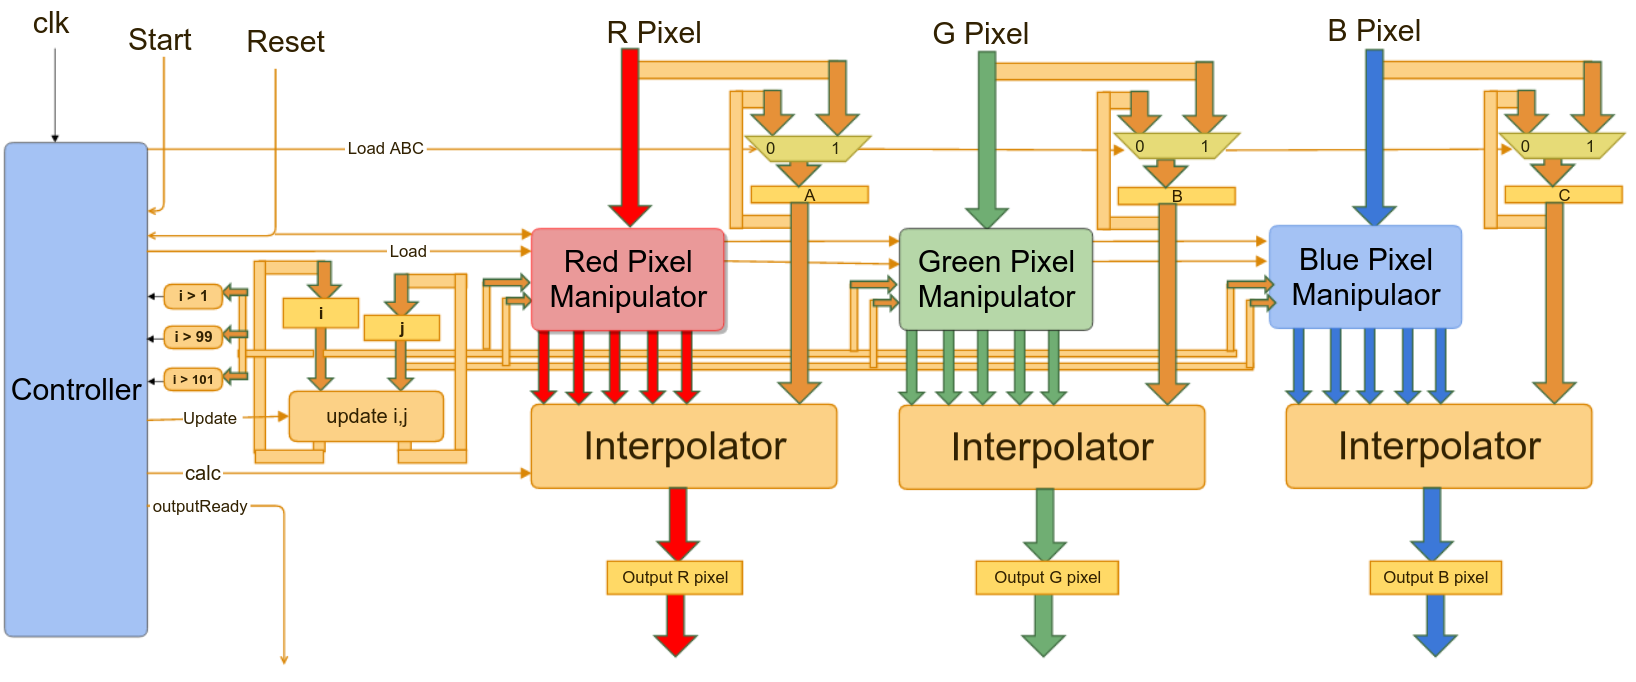
\includegraphics[scale = 0.45]{datapath.png}
	\caption{Stipulated datapath diagram}
\end{figure}
\end{landscape}

\clearpage

\vspace*{-3.5cm}
\section{Pixel Manipulator}
It consists of 4 vectors (numbered 0 through 3) consisting of 100 elements each where each element is a 16-bit number storing the pixel value. Everywhere, \texttt{i} refers to the vector/row number, and \texttt{j} refers to the element number in thar vector.
	
\vspace*{-0.1cm}
\subsection{Inputs}
\vspace*{-0.2cm}
When load is high, it reads 16-bits of Red/Green/Blue pixel from the input and also takes in the value of i and j from registers and reset and load from the controller.
\vspace*{-0.1cm}
\subsection{Functioning}
\vspace*{-0.2cm}
\begin{itemize}
  	\setlength{\itemsep}{-0.1cm}
	\item When reset is high, it sets all the entries in the vectors to \texttt{0}
	\item When load is high, it updates the \texttt{j\textsuperscript{th}} entry of the \texttt{i\textsuperscript{th}} vector to the 16-bit pixel value it takes as input
	\item When load is low, it updates the \texttt{j\textsuperscript{th}} entry of \texttt{i\textsuperscript{th}} vector to \texttt{0}
\end{itemize}
\vspace*{-0.2cm}
Note : Everywhere, the arithmetic in `i` occurs in modulo 4.
\vspace*{-0.1cm}
\subsection{Outputs} 
\vspace*{-0.2cm}
\begin{itemize}
  	\setlength{\itemsep}{-0.1cm}
	\item It outputs 5 16-bit values used by the calculator
	\item One of these 16-bit values is the current pixel value being processed (j\textsuperscript{th} pixel in {i-2}\textsuperscript{th} vector)
	\item Rest of the 4 values are of the adjacent pixels (which will be taken to be \texttt{0} in case they don't exist)
\end{itemize}

\section{Interpolater}
\vspace*{-0.1cm}
\subsection{Inputs}
\vspace*{-0.2cm}
It takes in five 16-bit numbers (C, u, d, l, r) from the pixel storer and another 16-bit number (K) as input.
\vspace*{-0.55cm}
\begin{gather}
\intertext{where,}
\vspace*{-0.2cm}
\begin{aligned}
 &C \text{  is the pixel value for which interpolated value is to be calculated}\\
 &K \text{  is the constant for interpolation and is equal to R, B or G respectively}\\
 &u, d, l, r \text{ are the pixel value of the adjacent cells (0 is they don't exist)}
\end{aligned}\notag
\end{gather}

\subsection{Outputs} 
\vspace*{-0.2cm}
\begin{itemize}
  	\setlength{\itemsep}{-0.1cm}
	\item When `calc` signal from controller is low, it's output is 0
	\item Otherwise, it outputs the interpolated pixel value which is caluated as below
	\begin{gather}
	output = round(K.a + \frac{(2^{16} - K).\frac{u+l+d+r}{4}}{2^{16}})
	\end{gather}
	\item This will use Full adders, Multipliers and Right Shifters.
\end{itemize}

\clearpage

\vspace*{-3cm}
\section{Updater (i, j)}
\vspace*{-0.1cm}
\subsection{Inputs}
\vspace*{-0.2cm}
It takes i \& j input from the registers and the `update` input from the controller.

\subsection{Outputs} 
\vspace*{-0.2cm}
It outputs two integers corresponding to updated value of i \& j. Basically it calculates them on the basis of traversal in the vectors inside the Pixel Mainpulators.
\vspace*{0.2cm}
\begin{lstlisting}[language=Python]
	if update = 0:
		updated_i = 0
		updated_j = 0
	else:
		if j = 99:
			updated_i = i + 1
			updated_j = j + 1
		else :
			updated_i = i
			updated_j = j + 1
\end{lstlisting}

\section{Pseudo Code}
This is the software implementation of our interpolation algorithm. The actual hardware implementation may vary. This is only for the red colour, it can be easily extended to the whole pixel.
\begin{lstlisting}[basicstyle=\tiny]
if reset = 1:
	set all of i, j, calc to 0
	set all values stored in pixel manipulator to 0

if start = 1:
	read value of A,B and C

while (i<102):
	if (NOT i>99):
		# read pixel values of RGB pixel and update jth entry of 
		# ith vector in all the three manipulators
	else:
		set jth entry of ith vector in all the three manipulators to 0

	RC = jth entry in (i-2)th vector in red pixel manipulator 
	Ru = (99 - j)th entry in (i-3)th vector in red pixel manipulator 
	Rd = (99 - j)th entry in (i-1)th vector in red pixel manipulator 
	Rl = (j == 0 ) ? 0 : (j-1)th entry in (i-2)th vector in red pixel manipulator 
	Rr = (j == 99) ? 0 : (j+1)th entry in (i-2)th vector in red pixel manipulator

	if (i>2 AND NOT i>101):
		outputReady = 1
		interpolated_R_pixel = round((R*RC + (2^16 - R)*((Ru + Rd + Rl + Rr)/4))/2^16)

	if(i > 101):
		outputReady = 0
\end{lstlisting}
Note : Everywhere, the arithmetic in `i` occurs in modulo 4.
\clearpage

\vspace*{-2.5cm}
\section{State Diagram}

In the initial state (given by state variable 0000), the reset is assumed to be high and start is assumed to be low.
This resets all the registers to zero and the controller variables `update`, `LoadABC` and `Low` are also low and the circuit is ready to start processing a stream of pixels.After one clock cycle, the reset still remains high and start remains zero indicating state 0001.\\\\
In the next clock cycle, the start input becomes high and reset becomes low which corresponds to state 0010.
The reset variable is assumed to remain low throughout afterwards.The start input remains high even after one clock cycle and the controller makes LoadABC signal high in the state 0011. When LoadABC signal becomes high, the coefficients iA, iB and iC are taken as input from the stream.\\\\
In the next clock cycle, the start and reset are both assumed to be low and the controller variable update becomes high. The update variable is an input to the block `Update i,j` which appropriately updates i and j.This variable is a function of load and the controller inputs i > 101. Also, the variable `Load` becomes high representing the fact that the first pixel values are fed into the inputs.These changes lead to a transition to state 0100.\\\\
Now, the variable `Update` remains high throughout until i exceeds 101.If the value of i does not exceed 1, the state remains same and this means that the circuit is taking input only. Therfore, the controller remains in this state for the 200 clock cycles (until the first 200 pixels are read) As soon as i exceeds 1, i.e. i becomes equal to 2, the state changes to 0101. Also, the contoller output calc is set high in this state representing that the interpolater block start processing the pixels.At this state, there are two processes happening, some pixel value is read and the required value for the pixel which was read 200 clock cycles before this pixel is computed.\\\\
In the next clock cycle, there is a transition to state 0110 where OutputReady varible becomes high denoting that the value at the output is valid.Thus, there is a delay of 201 clock cycles between the time of reading the first pixel and the time at which the first interpolated RGB value is ready to be output. The controller's state doesn't change until `i` exceedes 99. When i exceeds 99, i.e. after 10000 clock cycles when we statrted reading the input pixels, the state changes and in this state, the variable `Load` is zero as there are no more input pixels to fed to the circuit. For the next 200 clock cycles, when i does not exceed 101, the controller's state remains the same.\\\\
As soon as i exceeds 101, all but last interpolated values are computed and thus the variable `calc` is set to 0 which will get updated in the next state. The last interpolated value gets computed in this cycle and therfore OutputReady remains high in this state.In the next clock cycle, the outputReady is set to 0 which will get Updated in the next clock cycle. Also, during this cycle, the output of last interpolated value is done. In the final state, OutputReady is set to 0 as the output of all the interpolated values is done.

\clearpage

\begin{landscape}
\vspace{5cm}
\begin{figure}
	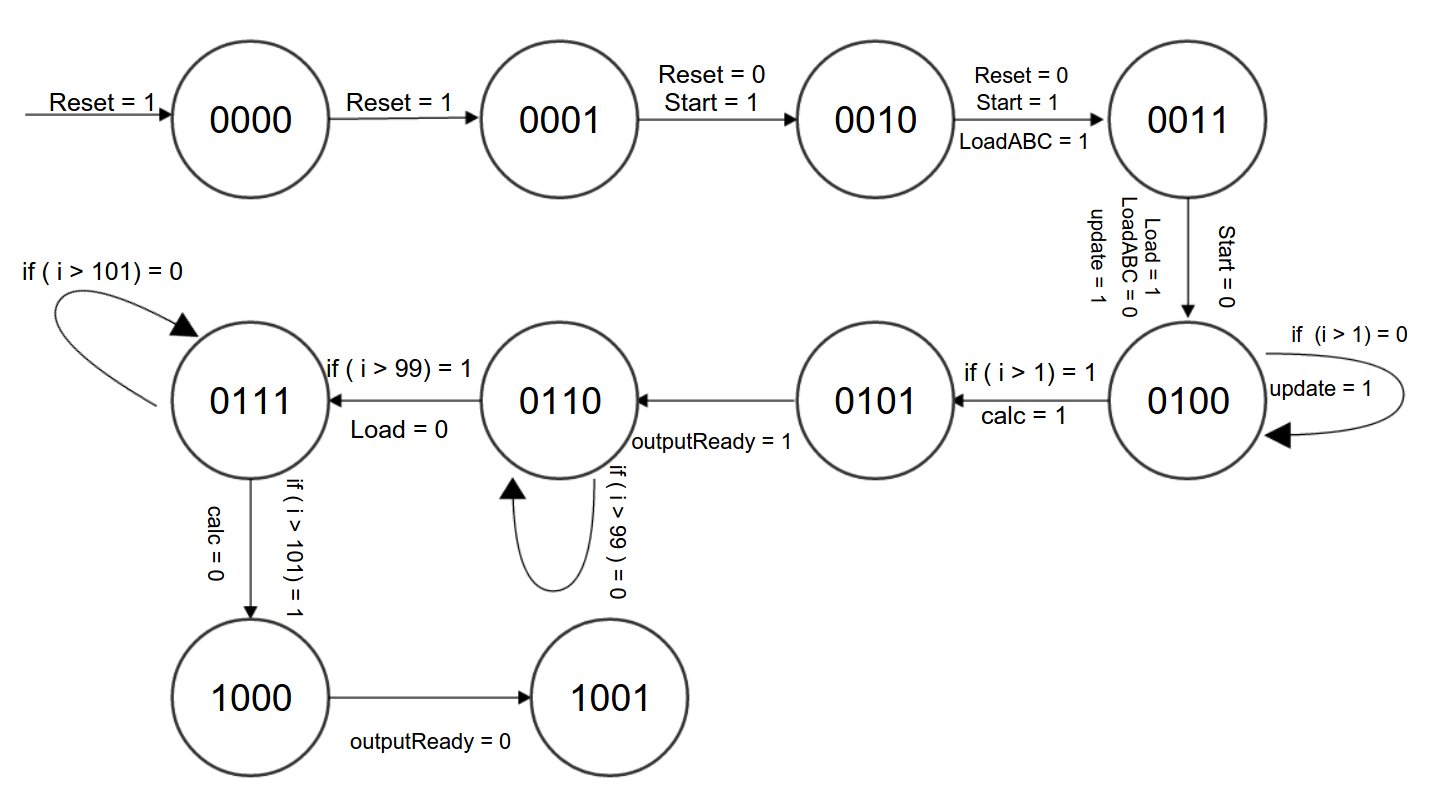
\includegraphics[scale = 0.43]{state.png}
	\caption{Stipulated state diagram}
\end{figure}
\end{landscape}

\clearpage
\vspace*{-2cm}
\section{Testing \& Verification}
We plan to test this program against real 100x100 images. We will convert them into RGB pixels and input them into our program, and do the reverse on the output of our program. Thus we can compare the the output image to see if it was correctly interpolated. This is an additional goal, and not part of our core project.

\section{Distribution of work}
Datapath will be implemented by Anuj Mittal and Shrey Rajesh. This includes implementing and testing all the black boxes i.e Pixel Manipulator, Interpolator and Updater block.\\\\
Controller circuit will be handled by Srajan Garg and Rishabh Agarwal. They will also do the verification and testing for the program by generating testbench from actual image data (hex dump) and qualitative analysis of program (blurring effect).\\\\
Preparation of test cases will be done by all the team members and the above tasks are also done in collaboration with other team members but the mentioned team members will mainly be responsible for above tasks.

\end{document}
